%pir api
PIR APIen er implementeret i PSoC creator. Top designet består af en input pin (P1[1]) der modtager et signal fra PIR-sensoren når der er bevægelse, se figur \ref{lab:pir_topdesign}. På figur \ref{lab:pir_topdesign_1} og \ref{lab:pir_topdesign_2} ses opsætningen af P\_PIR, den har en HW connection til isr\_pir og er indstillet til at have en pulldown modstand for at sikre at der står lav på pinen når der ikke er signal. Denne pin går ind og aktiverer en ISR routine. I main filen bliver global interrupt og pir interrupt aktiveret og i source filen ses det at selve ISR-funktionen går ind og kalder metoden ''movementDetekt();'' fra controlleren, der deaktiverer sprinkleren og starter en timer på 30 min, før der igen kan vandes.


\begin{figure}[htb]
\centering
{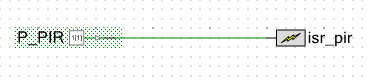
\includegraphics[width=0.60\textwidth]{filer/pics/pir_api_topdesign}}
\caption{Top design for PIR API i PSoC Creator}
\label{lab:pir_topdesign}
\end{figure}

\begin{figure}[htb]
\centering
{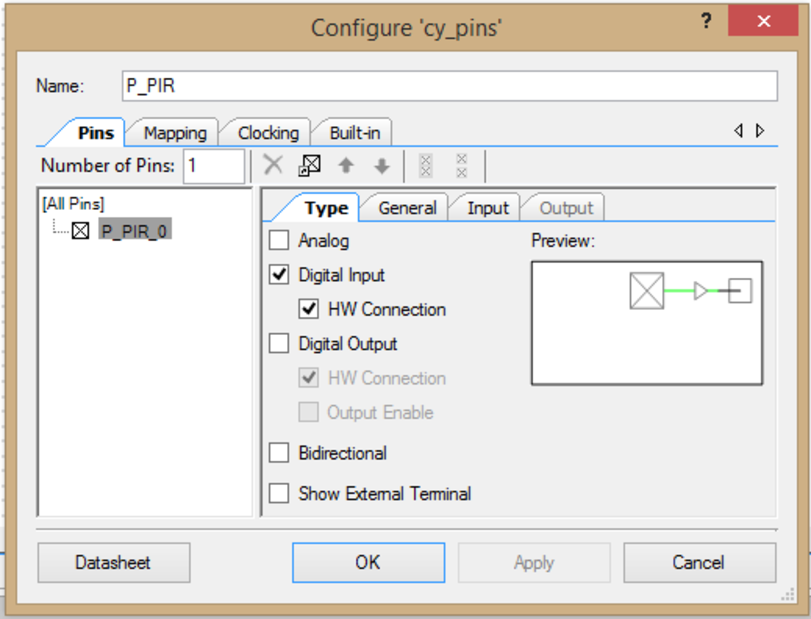
\includegraphics[width=0.60\textwidth]{filer/pics/pir_api_topdesign_1}}
\caption{Konfiguration af PIR pin i PSoC Creator}
\label{lab:pir_topdesign_1}
\end{figure}

\begin{figure}[H]
\centering
{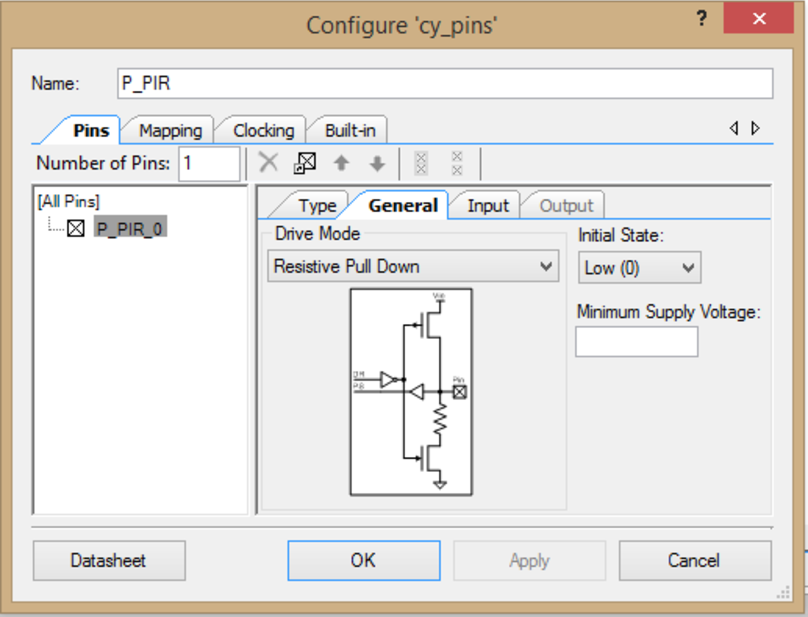
\includegraphics[width=0.60\textwidth]{filer/pics/pir_api_topdesign_2}}
\caption{Konfiguration af PIR pin i PSoC Creator}
\label{lab:pir_topdesign_2}
\end{figure}

\subsubsection*{Main fil}
\begin{lstlisting}[language=C]
int main()
{

    CyGlobalIntEnable; /* Her bliver global interrupts aktiveret. */
    
    isr_pir_StartEx(P_PIR); /*Her bliver pir interruptet startet*/
    
    for(;;)
    {
        /* Place your application code here. */
    }
}
\end{lstlisting}


\subsubsection*{Source fil}
\begin{lstlisting}[language=C]
CY_ISR(P_PIR)
{  
    loadData_movementDetekt();   
}
\end{lstlisting}